\documentclass[11pt]{article}

\usepackage[margin=1in]{geometry}
\usepackage[T1]{fontenc}
\usepackage[utf8]{inputenc}
\usepackage{lmodern}
\usepackage{microtype}
\usepackage{amsmath,amssymb}
\usepackage{graphicx}
\usepackage{xcolor}
\usepackage{enumitem}
\usepackage{float}
\usepackage{hyperref}

\hypersetup{
  colorlinks=true,
  linkcolor=blue!45!black,
  urlcolor=blue!45!black,
  citecolor=blue!45!black,
  pdftitle={From Spinoza to Grothendieck, missed opportunities for a category-theory-driven scientific revolution}
}

\setlist[itemize]{leftmargin=1.6em,itemsep=0.35em,topsep=0.35em}
\setlength{\parindent}{1.2em}
\setlength{\parskip}{0pt}

\newcommand{\quoteattr}[2]{%
  \par\smallskip{\normalfont\hfill--- #1\par\hfill\emph{#2}}%
}
\newenvironment{epigraphquote}
  {\begin{quote}\small\itshape}
  {\end{quote}}

\title{From Spinoza to Grothendieck, missed opportunities for a category-theory-driven scientific revolution}
\author{Hoapa project}
\date{September 2025}

\begin{document}
\maketitle

\begin{epigraphquote}
``And all science, \emph{when we do not understand it as an instrument for power and
domination}, but as an adventure in knowledge undertaken by our species through the
ages, is but this harmony, more or less wide and more or less rich from one period to
the other, which unfolds over the generations and centuries, by the gentle counterpoint
of all the themes emerging in turns, as if summoned from the abyss, to join and embrace
in her.''
\quoteattr{Alexander Grothendieck}{'Récoltes et Semailles', my translation and emphasis}
\end{epigraphquote}

In this text I will contend that, just like humanity with the global economy, the
research community is a prisoner and victim of the institutions organizing a game of
power and domination among its members. This situation doesn't stop the community from
thinking the next appropriate phase of its evolution, but it does marginalize and
disconnect the concepts on which it must be grounded. Namely, category theory---an
operational bird's eye view of mathematics---and its philosophical "extra structure",
whose systematic implementation in science would inject a healthy dose of:

\begin{itemize}

\item Perspectivism, as a methodological framework with a long tradition in philosophy to
which we append Grothendieck's "relative point of view" principle.

\item Concurrency, as in computer science: the art of solving problems by committee and
"message passing" strategies (what makes your multi-core processor work).

\item Legitimacy, trust and usefulness.

\end{itemize}

The words in the last item belong to a typically human domain of discourse, living on a
plateau of psychology. I will use a kind of translation device to make them operational
in science. This will allow me, as I explore the emergence of this rich network of
concepts in history, to conjecture an adjunction---a mutually beneficial, dynamic and
generative relation---between concurrency and perspectivism, itself a realization of the
well-known duality between ontology and epistemology.

Eventually, I will link this categorical or Grothendieckian scientific revolution with
the fate of humanity in evolution. Without it, it is doomed to destroy its environment,
if it doesn't destroy itself first (quantum computing being the most underrated
existential threat to date). Whereas a successful implementation of the simple yet
powerful and eminently democratic principles of concurrency theory, in research and
beyond, should invert the impact of new science and technology, from "automatically
weaponized and marketed" to safe and useful. This would in turn recalibrate and pacify
the global economy. Basically, an updated version of what Grothendieck said in his 1972
conference on research, using current ideas to discredit his own affirmation that his
mathematics were not useful for societal change and a reconstruction of interpersonal
relations.

\paragraph{Note.}

This text complements 'An introduction to Grothendieck's general theory of evolution',
which is exactly what the title suggests, and what the proposed scientific methodology
both understands ontologically and realizes epistemologically. These texts can be read
independently, this one being more adapted to philosophically minded readers
(mathematical concepts will be explained and illustrated in philosophy, but it also
allows the converse transfer of knowledge).

\section*{A Deleuzian Prelude: comparison between mathematical and philosophical practice}

Mathematics is like a unitary space which keeps on expanding with each contribution,
either in small increments in the case of a particular theorem pertaining to a known
region, or by opening new avenues made out of original problems, methods and
conjectures. In its most abstract form, mathematics organizes itself in categories (a
term borrowed from philosophy indeed), in which a mathematical entity is considered in
all its possible incarnations, from primitive to limit cases and all other interesting
specimens. They are conveniently represented by diagrams of dots and arrows, where dots
are cases and arrows are procedures explaining how to transform one into another. Those
containers of variability become extremely useful when we start building bridges between
them, and bridges between bridges, up to infinity, with the diagrammatic representation
coming along for the ride. In this framework, the space of mathematics doesn't lose its
unity, but it certainly gains the ability to shift perspectives on itself, to master its
own fluidity in order to adapt a level of detail, a style of contour or a color palette
to paint a specific problem such that the solution becomes obvious. Grothendieck was the
main architect of this approach, later dubbed "the relative point of view", also
grounded on "naturality", or the art of keeping things simple and flowing.

I will now use the term 'perspectivism' to refer to this method, which allows the
navigation of a space of knowledge, perspective by perspective, discretely or
continuously. With it, even logic ceased to be a fixed and primordial element, but
becomes a variable dependent on the topology, the changing parameters of the space
itself. Also, when I speak of category theory, I mostly mean Grothendieck's usage of it,
and focus on a particularly fruitful type of category: toposes. I also include the most
recent developments of this subject, \(\infty\)-toposes and their internal language,
called homotopy type theory. Fernando Zalamea puts it in those terms, and points to
where I would like to see those ideas flourish, outside of mathematics, and into
people's lives---the "science 3.0" this text documents:

\begin{epigraphquote}
``From a semiotical and philosophical perspective, the general method is fascinating: to
understand something, consider all possible points of view and search for a structural
connection between them. Only then you will be approaching true knowledge. A systematic
use of the liberty and multiplicity of topos theory in our ordinary life would have huge
consequences on tolerance, ethics, politics, and social action: an example of how high
mathematical practice would transform our everyday practice.''
\quoteattr{Fernando Zalamea}{'Grothendieck's 40 Main Years: A Unitary Vision Through the TSK Models'}
\end{epigraphquote}

In order to draw a parallel with philosophical practice, we must ask whether there is a
unitary space of philosophy, what would its dynamic be, and whether it has been equipped
with perspectivism in the above sense.

\paragraph{Note.}

\emph{I will put aside the claim that all of this has been achieved and recorded in
various oral forms all over the globe and quite a long time before the purported birth
of philosophy in ancient Greece, which is truly the birth of the European scholar.
According to the standard narrative, they appropriately ignored any previous and foreign
material and methodology, casting it as childish superstition, to establish a "novel
legacy", which has become the conventional space of philosophy in use today. While a
more refined and continuous history exists in the academic literature, the uniqueness of
Greece is nevertheless the norm, regardless of what was happening at the time in
Mesopotamia, Egypt, Persia, India or China, let alone in "uncivilized" regions. I
certainly do not mean to diminish the value of this legacy with those observations
concerning its origin---it is important however to remark the inability of the
university to correct the misconceptions which emerged in the service of its own
justification and the promotion of biased if not bigoted ideas of "progress" and
"civilization", severely narrowing its scope in the process. As I have alluded to in the
last section of the complementary text, this extended history would take us on a long
and winding path, which, interestingly enough, would nevertheless lead us to the same
realizations concerning concurrency, perspectivism and legitimacy, only with different
concepts and in different frameworks. Regardless, for the rest of this text, I will
remain within the domain of "Western" philosophy.}

An adequate spokesperson for the task at hand is assuredly Gilles Deleuze, who
forcefully engaged with the history and foundational aspects of his discipline. He would
certainly agree with the view of a space expanding by incremental contributions, as he
considered philosophical practice to be the creation of concepts, especially those so
important they would require "to be shouted" [le cri philosophique]. Regarding the unity
of the edifice, on the other hand, he repeatedly warned his audience during his seminars
that it was a mistake to pin one philosopher, or a unitary philosophical system, against
another in any direct fashion. This would only result in vain disputes. He addresses the
issue head on in his seminar of May the 20st 1980, when he compares Leibniz's infinitary
analysis with Kant's a priori synthesis, as systems. He concludes that a careful study
of what seems to be a "visible" contradiction shows that it is in fact a "hidden" but
explainable shift in the definition of an underlying concept (space and time in this
case, to which I will come back later). This seems to indicate he believes there is a
continuity between systems in the space of philosophy, albeit delicate, akin to the
network of mathematical concepts and their transpositions in category theory. In any
case, if it is feasible, it has never been systematized in philosophical practice. While
every mathematician is another Lego brick in the wall, every philosopher is, in effect,
an island. And if they are connected, the connections are hidden from view, submerged by
an ocean of "unprocessedness", that which Deleuze parted the time of a lecture. Can a
topos-like perspectivism emerge in such conditions?

Deleuze, following Nietzsche to which the term perspectivism is usually associated,
intends to reverse Platonism and to affirm the primacy of an immanent difference over a
transcendent identity, the Idea. A naive account of this project, sufficient for our
purpose, could depict it as a liberation from a framework of single and fixed points of
view on each object of thought and its derived hierarchy of all the "claimants", ordered
by their ability to comply with the Idea and point of view. In mathematics, this would
correspond to an (ordered) set theoretic view, precisely that which category theory
surpasses. According to both Rocco Gangle and Levi Bryant, or Dan Smith, this liberation
might be realized in Deleuzian philosophy:

\begin{epigraphquote}
``Deleuze conceives Ideas topologically as sets of variations or deformations in which
one form can pass into another while maintaining a structural identity, rather than as
fixed forms to which individuals more or less correspond.''
\quoteattr{Levi R. Bryant}{'Difference and Givenness: Deleuze's Transcendental Empiricism and the Ontology of Immanence' \& Rocco Gangle's 'Diagrammatic Immanence: Category Theory and Philosophy'}
\end{epigraphquote}

\begin{epigraphquote}
``Deleuze, however, often employs this `topological' method in his historical
monographs: when he interprets Bergson in terms of the concept of `difference' (as
formulated by Heidegger), or Leibniz in terms of a theory of `singularities' (borrowed
from Albert Lautmann), or Spinoza in terms of `univocity' (imported from Duns Scotus),
he is using a `foreign' concept, not explicitly formulated by the thinkers at hand, to
bring out aspects of their thought that might otherwise remain obscure.''
\quoteattr{Daniel W. Smith}{'The Doctrine of Univocity: Deleuze's Ontology of Immanence', chapter in 'Deleuze and Religion', ed. Mary Bryden}
\end{epigraphquote}

But while his approach to philosophical practice aligns with topology, group theory, the
Erlangen Program or structuralism à la Bourbaki, thus making the objects of study
richer, immanent and responsive to a multiplicity of points of view, it is not adequate
for a category-theory-driven philosophy "yet". The decisive step on the mathematical
side, epitomized by the Yoneda lemma, was the possibility to think each object
exclusively as a set of relations to all its neighbors, so much so that the interior of
the object could be safely forgotten. The object/concept becomes "pure modularity", in
the sense of engineering. Or, the extreme limit of the Hume-inspired empiricism of
Deleuze, where all is relation and relations are external to their terms. This "Yoneda
magic" is made possible by the guaranteed existence of a functor from the
well-established ground of set theory to the higher spheres of category theory and
\(\infty\)-toposes. Indeed, the lead actor in the categorical story is the functor, the
translation device going from one category to the other, a function taking a type of
structure as input and giving another as output, accomplishing the liquid unity of the
entire edifice and its navigability. It is hard to imagine the work of a
Yoneda-philosopher, one who would conceive his production of concepts not in terms of
their interior, but in terms of their modularity, where contribution and novelty are
never "breaks" but patient and continuous transformations of past contributions, and all
the possible paths between them, ad infinitum. Which is precisely the project of
\emph{homotopy type theory}, or how mathematicians who operate under the banner of the
nPOV---for multiple point of views---plan to record mathematics, physics and,
tentatively, philosophy, in a unified framework based on the last wave of Grothendieck's
mathematics (see ncatlab.org for more details).

What this text intends to expose is an implementable, open and autonomous version of
this: an information processing system in the form of a "scientific adjunction", or the
pairing of two functors, or "structure translations", whose ins and outs coincide so as
to form a loop, a generative virtuous circle between two organizations, whose data would
be collected by Yoneda-philosophers and encoded in homotopy type theory. I've listed the
two ends of this system at the top: concurrency and perspectivism, the former leaning on
the ontologic side and the latter, what this section is mainly about, in the epistemic
direction. The internal movement of such systems, between the two poles of probing and
encoding, can be looked at from different levels. Respectively (here progressing from
low to high level): [Yoneda-modularity \(\to\) concurrency \(\to\) ontology]
\(\leftrightarrow\) [homotopy type theory \(\to\) perspectivism \(\to\) epistemology].

I will now give three necessary and sufficient conditions for an information system to
be of the intended type, which I will now call 'Univocal Science':

\begin{itemize}

\item The system must be as presuppositionless as possible regarding the only two realms it
knows about, the Yoneda-probes and the world they are probing.

\item The system must be as separated as possible from the world it intends to depict.

\item The system must provide the most adequate language and data structures to its probes for
their deliberations and depiction.

\end{itemize}

The text will be pursuing those requirements, and eventually recover the components or
poles of the system. Going in reverse order, I will address the second item in the next
two section, and the first after that. As for the last item, if we believe the story to
be coherent up to this point, then homotopy type theory, as the internal language of an
\(\infty\)-topos, is the way forward. In practice, it would be like treating current
science as computer code and "refactoring" it, which is the last phase of software
development: basically "cleaning up the mess before you leave" and especially making
sure it's consistent with the rest of the system. It's arguably the most creative,
delicate and theoretically deep part of programming. This phase is simply ignored in the
university process, and only takes place "organically" when theories are adapted to be
used in practice.

I believe a crucial opportunity to be seized on this occasion, besides the obvious
unification across disciplines (or "learn once, write/read anywhere"), is also to make
scientific language customizable for the reader. That is, to consider data structures
for science that can \emph{record} very precise definitions in one unitary underlying
language (homotopy type theory), but which can then be \emph{read} in a multiplicity of
formats, with varying levels of details or styles, adapted to what readers are already
familiar with and their cognitive profiles. This amounts to a sort of inverse of the
pictorial metaphor I used at the top of this section to describe Grothendieck's
perspectivism, where \emph{problems} are presented in the most adequate way---in
programming lingo, we can imagine the recording phase to be conducted in assembly
language while the reading phase uses high-level language, the inverse of compiling. The
formalism of this duality would certainly extend another missed opportunity: literate
programming, as defined by Donald Knuth, which also avoids the necessity of
"post-production" pedagogical efforts, in this case by making the clarification of
purpose the first step. The central roles of homotopies (technically, continuous
transformations between paths in space) and functors (translations between structures)
would also make the whole system extremely flexible and able to systematize the
identification of correspondences between problems and solutions, even across very
"distant" disciplines---certainly making the charting efforts worth not just in terms of
usability, but of pure discovery. In sum, such a reworking of scientific and technical
language, especially when coupled with the "political" restructuring of the research
activity I will address in the coming sections, would assuredly see a fantastic boost in
both public engagement and quality of contributions.

This being said, in order to respect item one in the list and the autonomy of the
system, this framework can only be at best suggested to its users, who are entirely
responsible for its evolution and possible overturn.

\paragraph{Note.}

\emph{It appears that Deleuze didn't know about category theory, and certainly never
mentioned them, which is somewhat surprising for such an erudite polymath and a topic
which perfectly fit his intensions. Probably because his main mathematical sources were
Lautman who passed away before the categorical turn that he largely anticipated, and the
Bourbaki group who made a conscious decision to ignore category theory: despite seeing
its potential early on, they were already too committed to their structuralist and set
theoretic approach to re-found their own foundational work, maybe out of exhaustion, or
maybe out of pride, conservatism or some other human sentiment. In my opinion, this
missed opportunity is another sign of how the university-driven epistemic space is
unnecessarily fragmented, egotistically emotional, slow to update and under the
influence of social networks which are as political as they are academic. Also, as with
any institution, the intrinsic hierarchical structure interferes with the smooth flow of
information. What's more, while the research community is politically progressive in
general (and I will contend, due to the scholar's privileged front row seat to Nature's
inspiring opera), the functioning of universities is inherently conservative. The
seditious ideas which are the stuff of revolutions, scientific or otherwise, are always
fabricated in undercurrents, below the surface of the mainstream. (For example, the
extended evolutionary synthesis, which can capture biologically the traumas inflicted on
our organisms by capitalism and nationalism, is marginalized compared to the modern
synthesis, popularized by the selfish gene principle, which as the title suggests is a
modern update of the justification for social Darwinism.) I believe those flaws are
direct consequences of the economy of grants and publications, and expertise in general,
made all the more absurd by the "publish or perish" precept and the embedding of
universities in the erratic dyad of the global economy and the hierarchy of governmental
institutions. They are crucial in our collective inability to respond to the
environmental crisis, to update the prejudiced images of others emerging in people's
minds, to pacify this erratic dyad and to stop the proliferation of global existential
threats.} \emph{(A quick remark in passing, regarding the hot topic of AI: the above
list of requirements for an information system to implement perspectivism à la
Grothendieck is also the necessary and sufficient conditions for safe AI, especially the
second item, which is presented in the next section.)}

\section*{Leibniz \& Kant on space-time}

This section will mostly be giving a historical account of the fundamental break between
Gottfried Leibniz and Immanuel Kant, with references to current theories of foundations
of mathematics. Understanding "the system must be as separated as possible from the
world it intends to depict" as a simple principle of conceptual modeling stating that
the modeling activity should be entirely separated, or insulated, from any activity
happening in its object, I will claim that this principle is the actual reason for the
philosophical divergence.

\subsection*{From Leibniz's calculus ratiocinator\ldots{}}

\begin{epigraphquote}
``Leibniz reckoned that truth could only be determined in the bottoming out of our lines
of explanation, when the operational analysis halts, and where the intrinsic universal
character of the substance expresses its pure distinction from other substances and
aggregates. Thus, for Leibniz, substances are revealed through acts of demonstration in
extension. The concept resides in its potential exteriorization. In order to make sure
the demon is not deceiving us, we have to exteriorize our thoughts---which for him are
themselves made up of little perceptions, real substances---label them with symbols and
classify the combinatorial rules that specify how they compose with other ones. Once
this is done, calculemus, says Leibniz. We need to ``shut up and calculate'', we need to
prove statements in demonstration, through an iterative analytical process that may well
exceed our capacities of intuition. We need to exteriorize the vague and indistinct
concepts in our souls, actualize them in extension, and process them down to their
indubitable proofs of existence. Thus, the universal characteristic, a language that
encodes our concepts, must be combined with the calculus ratiocinator, the physical
machine, external to our minds, that processes the universal language. He thought that
by crunching the numbers on such a sophisticated machine, even the most subtle
metaphysical questions could be distilled to their bare distinctions. The point of
exteriorizing this process and not just calculating in your head, was that we needed to
make sure we were not deceiving ourselves: in this way, we could check the proof, and
locate any errors.''
\quoteattr{Alexander Wilson}{'On Something Like an Operational Virtuality'}
\end{epigraphquote}

Following the lines of our structural ontology-epistemology duality, this enterprise of
exteriorization is the practical conclusion of Leibniz's theory of knowledge, based on
the idea that all truths are analytic, that every determination is ultimately
conceptual. It is grounded on his mathematical method of calculus, which would allow the
daunting task he set for himself to be completed, as well as his ontology, itself
composed of a series of principles such as the Identity of Indiscernibles,
Pre-established Harmony or Universal Expression, describing a universe that is saturated
and as perfect as can be. It is made out of monads, each of which expresses the entire
universe, but does so in its own way, according to its particular clear and distinct
zone of expression. This theory of monads is a landmark in the development of
perspectivism in philosophy and a source of inspiration for our own construction here,
but not what we need. A number of adjustments are necessary, especially a detour via the
dual notion, synthesis.

The exteriorization endeavour cited above is precisely what led a "classical"
mathematician, one who had observed the calculemus dictate, Vladimir Voevodsky, to
switch and embrace "constructivism", the stronger but more demanding practice emerging
naturally in homotopy type theory and \(\infty\)-toposes. His motivation was eminently
pragmatic: a mistake was found in one of his papers, long after it had been accepted and
acclaimed. He concluded that peer-reviewing in this field was getting too intricate for
the human mind, and proof checking by computers was necessary. In so doing, he was
driven to join the nPOV category theorists into their efforts to found mathematics on
the set of ideas I've been referring to throughout this text. The technical and
mathematical aspects which necessitate the switch are fascinating and transport us from
a Leibnizian-analytic to a Kantian-synthetic world. They are beautifully summarized by
Robert Harper in the introductory lecture to his course on homotopy type theory, stating
that the ``synthetic perspective on mechanized reasoning'' is strictly superior to the
analytic counterpart in terms of efficiency, strength of results and beauty, and
insisting that it is so contrary to "common wisdom".

\subsection*{\ldots{}To Kant's synthesis}

Leaving those mathematical considerations aside to concentrate on the philosophical
stream, let me come back to Deleuze's seminar mentioned above, when he compares
Leibniz's and Kant's theories of knowledge. According to Deleuze, Leibniz starts with
the most evident of tautologies: 'A = A', whose philosophical formulation is 'all
analytic propositions are true'. He then proceeds to reverse the principle: 'every true
proposition is necessarily analytical'. This is the starting point of a formidable
philosophical project, creating an infinite universe where every fragment of it contains
the whole. In its limit, he has trapped all events in an exhaustive ontology of divine
creation, which is then entirely replicable in his epistemology thanks to calculus.
However, like the pessimistic view on what a mathematical proof is, there is nothing new
once the formulas have all been laid out in order, nothing that wasn't already present
in the original maelstrom. One can at best enlarge their own clear and distinct zone of
expression, but the global space, already as perfect as can be, stays the same. Contrary
to Kant, it doesn't leave any room for a novel, foundational event on the epistemic
side. This is how the Kantian revolution, the emancipation of a pioneering subject,
opens new avenues, notably into "everything aesthetics". In the limit, ``knowing is
creating a synthesis because it necessarily means leaving behind all concepts in order
to affirm something extra-conceptual in it'', according to Deleuze. Maintaining that
this dissonance is not a matter of right and wrong but how each philosopher construct
their system, he points to a transformation that is antecedent to and constitutive of
the visible analytic-synthetic chasm, a critical but hidden metamorphosis applied to the
concept of space and time by Kant (influenced by Hume), in opposition to the canonical
notion which had been consensual since the Greeks, mostly upheld by Leibniz---space and
time are "only" relational and ideal entities and do not exist outside of the things in
the world.

With Kant, preparing his concept of the transcendental subject, space and time are
forms, forms of exteriority and interiority respectively. That ``through which
everything that is exterior to us reaches us'', and that ``which happens to us as
interior, interior to ourselves'', such that ``the thinking subject is pure form of
intuition'' where 'form' is to be understood roughly as structure, or rather
"structuring". And that which is being structured, and in a particular sense realized in
phenomena, is reality itself. In effect, in order to enrich the notion of the subject,
Kant needed to "unblend" space-time and each thing or agent's concept. Understanding the
role of the transcendental subject, synthesis, as a kind of modeling activity, composed
of "probing" (as ``receptive sensibility'') and conversely "rendering" (as ``active
understanding''), this shift in the conception of space and time can be reinterpreted in
simple terms by the requirement that any such activity, to be conducted optimally, must
be an insulated event, separated from any other event. Hence the 'transcendental'
terminology of Kant, or the general sensation that our minds are separated from the
world and even our own bodies. It also works for genetic processing, whose modeling
activity can be effectively transposed from cells to computers, because they're not
dependent on the specificities of their "hardware". Likewise, ``computers might as well
be made of green cheese'' according to Samson Abramsky. With this generalization, we can
affirm that the practice of science by humanity, as a special event and a modeling
activity, must follow this pattern.

Time permitting, we could find other reasons to believe human science is another
installment in a series of such natural information processing systems, emerging in
turns in the evolutionary process, parameterized by what their existence requires and
what they make possible in their context, or alternatively what they take as input and
give as output, while being unreasonably well defined by their mathematical properties.
(This is the main theme of the complementary text on generalized evolution.) A
categorical classification of such systems, as special events, could be based on group
theory (and maybe shed lights on the ubiquity of groups in physics):

\begin{epigraphquote}
``Classifying geometrical objects by their degrees of symmetry represents a sharp
departure from the traditional classification of geometrical figures by their essences.
While in the latter approach we look for a set of properties common to all cubes, or to
all spheres, groups do not classify these figures on the basis of their static
properties but in terms of how these figures are affected (or not affected) by active
transformations, that is, figures are classified by \emph{their response to events that
occur to them}.''
\quoteattr{Manuel DeLanda}{'Intensive Science and Virtual Philosophy', his emphasis}
\end{epigraphquote}

Turning back to the philosophical debate, what then is left of 'A = A', which seemed
like a definitive proposition? According to Johann Fichte, a disciple of Kant (and still
following Deleuze's account), it is not so and must be corrected into 'A = A, if A', a
hypothetical proposition. Taking the transcendental subject as the nexus of all
philosophy, ontology and epistemology included, he declares the primordial proposition
to be 'ego = ego'. This is where and how this text and German idealism part ways,
bypassing what would be a long and tedious historical analysis of how the glorification
of the transcendental subject served as justification for the new political order, which
transitioned from land-ownership to time-ownership in order to accompany the weaponizing
and marketing of the fruits of the first scientific revolution, by then ripe for an
(uncontrolled) economic boom and colonial expansion, which directly led to the current
ecological crisis and existential threats.

We will contrast Fichte's extension to that of Voevodsky, the univalence axiom: '(A
\(\cong\) A) \(\cong\) (A = A)', or 'equivalence is equivalent to equality'. This is a
necessary axiom for the eminently Kantian project of a "synthetic foundation of
mathematics", to be added, very much like a keystone/cherry on top, to Grothendieck's
last wave of mathematics---a program started with his seminal letter to Daniel Quillen,
'Pursuing Stacks', and related texts. (Interestingly, it took the mathematics community
almost 30 years to really get started from those foundations. They did only after
homotopy theorists and type theorists realized they had been working on the same
material all those years without realizing it---something which would have transpired
much sooner, had they properly "refactored their code" and shared their problems). In
the following sections, I will be using Voevodsky's formula to motivate the use of
concurrency as part of our "scientific adjunction", Univocal Science, after another
detour into Grothendieck's methodology.

\paragraph{Note.}

Using Deleuze again, and in order not to deter future readers, I will greatly accelerate
``the velocity of thought'' in the next two sections.

\section*{Grothendieck on solitude}

I will now quote from the opening pages of his mathematical memoirs, where he recalls
his relationships to school and mathematics in the years prior to his encounter with
"real" mathematicians in Paris (plural because his discovery of mathematics was almost
entirely autodidactic). In this he will let us know what kind of transcendental subject
he is. First, let's note that with his uncanny attention to details, he offhandedly
extracts the locus of the philosophical debate above, of which he was most probably
unaware, in a parenthesis:

\begin{epigraphquote}
``It was the book's problems, not my problems. Even though the truly natural questions
were not in short supply. Thus, when the lengths a, b, c of the three sides of a
triangle are known, this triangle is known (apart from its position), so there must
exist an explicit "formula" to express, for instance, the area of the triangle as a
function of a, b, c.''
\quoteattr{Alexander Grothendieck}{'Récoltes et Semailles', my translation and his emphasis, ibid for all quotes in this section}
\end{epigraphquote}

In his own words, 'Récoltes \& Semailles' is about the creative process. Such as here,
talking about the necessity of questioning fundamental notions, the volume of a solid in
this case:

\begin{epigraphquote}
``It is in this act of "superseding" [passer outre], in short of being oneself and not
simply the expression of a law-making consensus, of not staying circumscribed within the
imperative circle it fixes for us - it's above all in this solitary act that one can
find "\textbf{creating}" [la création]. Everything else comes as an extension.''
\end{epigraphquote}

In this manuscript, of the 42 mentions of solitude all but 3 are directly associated
with work. What transpires from the text is that solitude for him is not so much a
necessary condition for doing mathematics, as it is \emph{made} imperative by the
irreconcilable discrepancy between perspectives on how mathematics should be carried
out, between him and absolutely everybody else. In contrast to the "Yang" attitude of
his colleagues, their desire to solve the hardest problems at all costs, without regard
for the mathematical edifice, and where mathematical output is used as a ranking system,
he insists on attention to details, elegance, naturality, the place in the overall
architecture of each element or "what the mathematical things tell him". It is this
rupture, or rather this nonconnection, which really forced him to work in isolation.

With a distinction between numerical and political solitude, we can now preserve a
remarkably creative, synthetic and foundational modeling practice from obstructive
events, while opening the process to concurrency (especially since the reformulation and
customizability of scientific language should draw a new enthusiasm). Also, there is
nothing manifest in Grothendieck's vision that prevents a multiplicity of actors from
working on a problem. If anything, his own perspectivist methodology and favorite
concepts, such as sheaves, seem totally adequate (and indeed can model concurrency
itself). But only if the working community respects the "sanctity of the modeling
event":

\begin{epigraphquote}
``From the limited experience I had gathered then, it seemed that I was the only soul in
the world bestowed with a curiosity for mathematical questions. [\ldots{}] There wasn't
in me a shadow of a doubt that I wouldn't succeed, that I would fail to find the final
words in the story of things [le fin mot des choses], provided that I only went to the
trouble of scrutinizing them, by spelling out what they were telling me, as I went
along. The intuition of, say, volume, was indisputable. It could only be the reflection
of a reality, elusive for the time being, but perfectly trustable. It was this reality I
needed to capture, quite simply.''
\end{epigraphquote}

The passage from the lonely soul 'I' to an enthusiastic 'we' is the subject of the next
section, but already the contemplative reader can get a feeling for how the formula
'equivalence is equivalent to equality', '(A \(\cong\) A) \(\cong\) (A = A)', is a
gateway to adaptable and cohesive communities.

\section*{*'s Spinoza on the infinite}

\begin{epigraphquote}
``[T]here are two ways of identifying what is an attribute: either one looks, a priori,
for qualities conceived as unlimited, or, setting out from what is limited, one looks, a
posteriori, for qualities that may be taken to infinity, which are as it were "involved"
in the limits of the finite''
\quoteattr{Gilles Deleuze}{'Expressionism In Philosophy : Spinoza'}
\end{epigraphquote}

I used the star sign in the title to express how Spinoza's perspectivism is in a sense
built-in in the system, which is responsive to all kinds of interpretations (but not an
"anything goes": perspectivism is not relativism or subjectivity, and Spinoza's
entangled network of concepts requires conscientious extrication.) I'm mostly interested
in Deleuze's, Peirce's and Spinoza's Spinoza. They all give a remarkable philosophical
sketch of the ontology-epistemology adjunction forming what I've referred to as
"Grothendieck's generalized theory of evolution", realized in parts in 'Difference and
Repetition', pragmaticism or 'the Ethics', respectively. The core of this depiction is
an interface, a kind of asymmetric yet faithful mirror, between the realms of the finite
and the infinite, making both of them possible and necessary. I believe the key is the
mastery of presuppositionlessness by use of the infinite (the most costly assumptions
are always the boundaries), coupled with the "untaming" of the absolute infinity: the
art of letting it run far and, more importantly, wide---and in a sense, free of our
assumptions and limitations. Still, the brilliance of Spinozism lies as much in its urge
for joy and freedom, its "politosophy", as it does in those metaphysical contemplations.
Ultimately, it is the embrace of those two poles.

The univocity of being, or the ontological stance that 'being', the verb to be, can be
said of all things equally or equivalently (which is equivalent if we believe
Voevodsky), may they be a rock, an animal, Nature and/or the absolute infinity.
Spinozism implements univocity by virtue of being a system in which all things, or
participants, have the same relationship to the system as all the others: all things are
endowed with an infinite number of extensive parts which behave according to a certain
relation and express the essence of the individual thing, and so on and so forth\ldots{}
the immense diversity of beings are all captured in the system under a unique type. (Or,
at a low mathematical level, a non-exhaustive set of general instructions for how to
construct things and how they should behave/respond to events, universally
applicable---the essence of the geometrical method). The role of the attributes and its
further complications is to make the finite "layer" concur with the infinite. Which is,
as the history univocity shows, both the real conceptual difficulty and an important
point of political contention, between univocal liberators on the one side, and
supporters of the analogical doctrine, which justifies the established hierarchy of
"Scala Naturae", on the other---we recover the two poles above, politosophy/politics and
metaphysics, and their intimate relation. (A third group, following an equivocal
interpretation, represents a path through philosophy going from negative theology to the
Frankfurt School via Hegel and Marx, with Bill Lawvere serving as the
"mathematician-extractor", which I have ignored in this text but can nevertheless
further substantiate my claims, albeit not as efficaciously.)

\begin{epigraphquote}
``Thus we come to the core of Spinoza's immanent metaphysics. [\ldots{}] There are no
absolute cuts between one thing and the next in Spinoza's metaphysics, only more or less
attenuated relations corresponding to variable degrees of commonality. Such relations
(the affects and common natures) are themselves constitutive of higher-order entities,
in such manner that the boundary between relatum and relatio is always at best localised
and relatively unstable. To put it in more Spinozist terminology, the clear conceptual
and systematic distinction between modes of substance on the one hand and the affects
and common natures that structure these on the other does not in fact differentiate two
separate real types of being but rather provides complementary perspectives on infinite
substantial expression itself. What is, is expressed as structure. Ontology is just
local metaphysics.''
\quoteattr{Rocco Gangle}{'Diagrammatic Immanence, Category Theory and Philosophy'}
\end{epigraphquote}

Besides, to give just one argument among a multitude and assuming that the
\emph{possibility} of using concurrency in an epistemological system have been
established in the previous section, I will further contend that it is a
\emph{necessity} because it is "pure decentralization". If it is placed at the "center"
of the system, as a sort of distributive mechanism, then the system stays decentralized.
And it must be or else this center becomes an obtrusive event. Conversely, concurrency
delivers a multitude of engineering perks which are just about as essential for our
purpose. This student of Deleuze also finds traces of it in the "higher spheres" of 'the
Ethics':

\begin{epigraphquote}
``I would like to emphasize the fact that in the \emph{Ethics}, when Spinoza says: "I
don't understand", \emph{intelligo}, he says "I". When he wants to cite an example, he
says Paul or Peter. And when he says: "we feel and we experience", it is a "we" who
matter. That means: it's all together. In the same way, when he talks about the
intellectual love of God in book V, it is: \emph{omnium}, it's all together.'' Deleuze's
seminar of March 17, 1981, adapted from 'The Deleuze Seminars' transcript and
translation
\quoteattr{An anonymous student}{}
\end{epigraphquote}

Now, there is one particular model of concurrency which also happens to respect the
principle of univocity/unique types: the actor model. As a model of computation itself
inspired by fundamental physics it's not surprising to see it appear in our metaphysical
discussion. In brief, in this framework computation emerges out of the conversation of a
large number of actors, which are really just mailboxes. They can receive and send
messages, decide how to respond to future messages and create new actors. An
implementable, autonomous and open science can be naturally designed from this set of
actions if we integrate them in a \(\infty\)-topos architecture, where actors are not
individuals but conversations between individuals. We use Voevodsky's univalence to
ensure all participants consider each other as equals and, at the same time, the system
accepts as much diversity as possible. (This set of actions is already what scholars do,
except in a closed and bloated implementation with high dependency costs, primarily as
ranked ever-applicants instead of team-first conversationalists---just like once-free
workers in capitalism.)

A compact slogan, to aggregate the set of conditions we've accumulated for our Univocal
Science so far (optimal language, insulation, univocity), could be: "don't multi-type
your probes, only multi-type your concepts, and make everything Yoneda-modular". Or in
ordinary language: "don't put people in boxes (consider all of them as, say,
philosophers), put the fruits of their collective reflection in boxes, and make sure all
of that can communicate and be communicated efficiently." Or, from the point of view of
the information system: "the system wants to record and classify all the concepts and
all their relations, but it wants to know as little as possible about the probes and
can't classify them".

\subsection*{Diagrammatic interlude}

To help with the discussion in the next section, I observe univocity is also naturally
realized in the realm of category theory, since every mathematical concept can be
alternatively and equivalently thought of as (with diagrammatic representation):

\begin{itemize}

\item an object of a category : an island of stability in a sea of variations---variations on
a concept\\ (dot)

\item an identity morphism in a category : a variation which loops on itself, achieving
stability\\ (small looping arrow starting and
finishing on one dot)

\item a category : an archipelago we decide to treat as an object, encapsulating a singular
concept in all its variations\\ (large circle
enveloping dots and arrows)

\item an identity functor / endofunctor : a vast current/translation between archipelagos,
which in this case loops back around one archipelago---where archipelagos are surrounded
by an ocean of currents/translations, called
functors\\ (large looping arrow)

\item any morphism or functor : when we "deloop" the identity arrows, by relaxing, or
"forgetting" the requirement that the origin and target of the arrow should be the same
(they could just be "equivalent enough"), then all arrows are mathematical concepts in
some sense, and vice versa\\ (arrow or dot)

\end{itemize}

\ldots{}Depending on the point of view adequate for the context. The pattern can
continue towards more and more generality, diversity, detail\ldots{} to infinity,
according to the kind of category theoretic operation we iterate over. Infinity-toposes
are of this kind, where the number of ways in which things can relate to each
other/themselves are unbounded, which, again, is optimal for recording concepts and
forming a unitary space of philosophy, or science in general. Crucially, thanks to the
very nature of homotopies, no matter how wide/diverse it gets, this space would be as
compact as can be. Univocal Science is "manageable".

\section*{(Peirce \& Martin-Löf) on diagrammatic trust}

\begin{epigraphquote}
``[L]ogic has, not only an ontological layer and an epistemological layer, but also a
deontological layer underlying the epistemological one.''
\quoteattr{Per Martin-Löf}{abstract of 'Logic and Ethics'}
\end{epigraphquote}

Taking those logician-philosophers as dynamical systems:

\begin{itemize}

\item Charles S. Peirce takes as input \(\ulcorner\)Kant and Spinoza\(\urcorner\) and outputs
\(\ulcorner\)a logic Martin-Löf will be taking as input\(\urcorner\) and
\(\ulcorner\)pragmaticism\(\urcorner\)---a practical framework for clearness of mind
which is a distant relative of Grothendieck's methodology and our scientific adjunction.

\item Martin-Löf takes as input \(\ulcorner\)the failures of logical positivism\(\urcorner\)
and \(\ulcorner\)the infancy of logical intuitionism and mathematical
constructivism\(\urcorner\) and outputs \(\ulcorner\)the type theory for homotopy type
theory\(\urcorner\)---that which naturally emerges in \(\infty\)-toposes.

\end{itemize}

"Deontology" and "trust" surface regularly in Martin-Löf's writings, especially in
reference to Peirce and around the concept of assertion, evidently fundamental for
logic. They do make the historical process we've been following continuous, but in this
section I will not be using material coming directly from the title philosophers.
Instead I will describe a category,
\(\langle\!\!\langle\)Politosophy\(\rangle\!\!\rangle\), and its diagram, whose dynamics
is based on usefulness, trust and legitimacy. It is isomorphic to the category which is
generated by the scientific adjunction and includes Univocal Science, meaning roughly
that they're equivalent enough to be interchangeable. The objects of
\(\langle\!\!\langle\)Politosophy\(\rangle\!\!\rangle\), its islands, are large-scale
organizations of humans, and arrows/currents are historical shifts from one organization
to another.

At this political level which will become relevant for our purpose, I would like to
oppose the freedom-denying assumption that those objects are legal systems and the
arrows more or less concerted reforms of those systems. This is a Top-Down view that
adds unnecessary structure that is only correct if you assume, in the D-T direction,
absolute compliance with the rules and a total coverage of all activities by them (what
we are pressured into), and in the T-D direction a miraculous form of government, as if
the whole was really the top (the dystopian utopia, or vice versa). Despite the
heterogeneous efforts of oligarchies worldwide, it is not the case, and has never been.
Only the bottom-up view is conform to reality. Even if they tend to gain stability over
time, governments are always at best tolerated. As for the "industrial civilization", it
is now in a position of monopoly because it is slowly killing its main competition,
networks of solidarity (which hide a wealth of complexity behind its main entryway,
attachment, as in attachment theory in ethology and psychology---the initial building
block of humanity). Like a virus is not part of the cell it infects, capitalism is not a
native element of a "terminal object".

Our goal here is to locate \(\langle\!\!\langle\)Politosophy\(\rangle\!\!\rangle\)'s
"terminal object", which is, in terms of arrows, the nexus of the category where all the
currents ultimately land, or the Rome to where all roads lead. It can be interpreted in
two ways: primarily as the end result of an internal process, or conversely as the start
of something new and external. As we'll see, this special object is isomorphic to
Univocal Science, viewed as an element of \(\langle\!\!\langle\)Epistemic
systems\(\rangle\!\!\rangle\), using the same concurrency-to-perspectivism structure,
but with different purpose and conditions.

First, let's build a mental image of the diagrams of the categories by considering the
following funnel-shaped energy landscapes\textsuperscript{1} representing how proteins
get folded according to the "principle of minimal frustration". And how they can also
represent the history of engines, which will be the introductory example for how those
diagrams work:

\begin{figure}[H]
  \centering
  \IfFileExists{../communication_drafts/figures/energy_landscapes.png}{%
    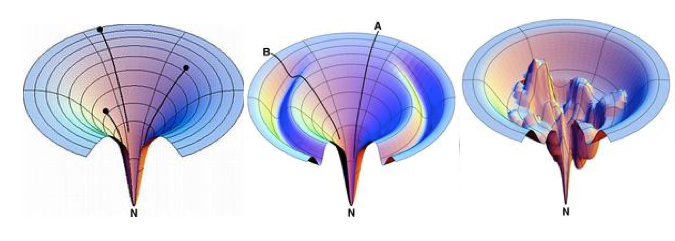
\includegraphics[width=0.88\linewidth]{../communication_drafts/figures/energy_landscapes.png}%
  }{%
    \fbox{%
      \begin{minipage}[c][1.8in][c]{0.82\linewidth}
      \centering\small
      energy landscape referenced in the Markdown source.\\
      \emph{The image file was not present at compile time.}
      \end{minipage}%
    }%
  }
  \caption{energy landscape.}
\end{figure}

N is for native state, the intended configuration useful for the cell, which is achieved
chemically because it corresponds to the state maximizing entropy and minimizing free
energy. You can think of the evolving configuration of the protein as a ball rolling
down the side of the funnel under the force of gravity, as it would if it was in your
living room. Additionally, configurations can go over ridges via catalysts, special
chemical reactions which can defy entropy/gravity.

Now, swapping proteins for types of engines, I state that entropy/gravity is usefulness,
the ultimate metric, that which must be maximized. Or more accurately, usage, a
difference between positives and negatives. Optimizing usage will always attract rolling
balls downwards, that is provoke new engine configurations, a constant flow of technical
development. A further condition for improvement, what makes the descent into optimized
usage possible, is the internal level of trust between each part of the engine: how
solid the connection between, say, the piston and the crankshaft is, how much pressure
they can resist, how fast they can go without losing cohesion or disintegrating. Usage
takes you down, but internal trust is what makes you stick to the wall. The wall is your
integrity, it is where trust makes existence possible.

In the first image on the left, any configuration you start with will take you directly
to N, and like the salad spinner, the ideal system is found directly and it will stay in
this happy state forever. It makes for a very simple category with only one possible
target object. In the next diagram, B is like the steam engine, it reaches a point in
its evolution when no modification to internal trust can be an improvement for usage. It
finds itself stuck in a furrow of legitimacy: it is the most efficient of its kind, and
as far as, say, 1870 engineering can see, it is N. This is when another kind of trust is
necessary, a catalytic trust which ignores deleterious modifications for a while until
the system finds itself in a whole new valley closer to usage paradise, with brand new
internal trust strategies. With B going over the hump, this category has two target
objects, where the steam engine object also has an arrow to N (which was the combustion
engine for a while but has now many competitors---we might be changing valleys again).
The final diagram represents a more realistic or "organic" category, with many objects
and arrows.

To get the category \(\langle\!\!\langle\)Politosophy\(\rangle\!\!\rangle\) from the
sketch above, we can simply reinterpret the words associated with the objects and
arrows. It is straightforward for usage, legitimacy and trust since in the social and
political realm they recover their usual meaning. We can distinguish between internal
trust, which would be the practical and immediate cohesion of a group, from catalytic
trust, which would be their ability to figure out and formulate the best organization,
adopting usage as the metric and trust as a condition for existence. In both cases, we
recover what politics is supposed to be, and whose current state of affairs is simply
degenerate, both in practice and in its theoretical output. (Here we can use Spinozism
or applied category theory to make those judgement calls "under the hood", and in both
cases, compositionality is utterly broken in politics/economy).

This situation is hardly surprising given that the main metric is "investability" (which
is related to but even worse than profit), and that trust is replaced by control. We are
barely touching the wall of the funnel at this point and there are no positive solutions
in sight in this direction. In diagrammatic terms, the arrow we're following goes to
\(\emptyset\), false or more appropriately, absurd. Or we could say, following
leibnizian perspectivism, that our "particular clear and distinct zone of expression"
doesn't seem to include a sustainable organization (freedom preserving, fair, non
violent). Which would be a hopeless situation for us if we believed in the reality of
the freedom denying top-down view and its degenerate dictionary for gravity and
integrity. And as long as we do, it is.

Fortunately, the category is not broken, only our perspective and metrics. Given the
capacity and history of the concepts weaved into the web of equivalences I have exposed
so far, we can be confident a healthy dose of sincere catalytic trust modeled after
Grothendieck's methodology will point to an adequate and natural design for social
organizations. As it does, by isomorphism, with science practice.

Together, this organization and Univocal Science would coexist in another mutually
beneficial relationship, and become harbors for each other: the best place to do and
formulate the other, respectively. Just like their inverse images, governments and
finance, they're a "couple". If implemented properly, the social system brings public
engagement and quality of contributions to science, and science prepares the very
detailed map of the ecosystem social organizations need to pacify their relationship to
their environment. This relationship would be mutually beneficial as well, completing an
evolutionary sound virtuous cycle (again, to be contrasted with the weaponizing and
marketing of all technologies).

The following quote will illustrate how Grothendieck's methodology and principles
realize in mathematics the catalytic trust of our diagrams. Here the question is how
"universal properties" of category theory can replace efficiently a heavy "low-level"
logical machinery, only if one is willing to blindly trust some intermediate steps. It
contains some jargon which can be safely ignored, the trust element transpires through
the natural language alone:

\begin{epigraphquote}
``We can have a "categorical version" which consists in saying that, concretely, it
falls under a principle "à la Grothendieck". For instance when one demonstrates that an
ultraproduct of fields is a field, one makes an inductive limit of projective limits,
but the partial projective limits one takes are not really fields because they are
products of fields, so it "exits [its definition]". But in the limit it becomes a field
again. So, in effect, we make a universal construction, and allow ourselves to pass
through things which [...] are not representable. Here I would say there is a
methodological substitute to the use of ultraproducts, which would be this principle of
Grothendieck (one of them): in constructions we are allowed to pass through non
representable steps, and to interrogate representability at the end.''
\quoteattr{René Guitart}{from his talk 'Theory of the theory: esquisse or topos?', ENS, 01/14/2006, my translation}
\end{epigraphquote}

Grothendieck advocates the usage of "unreal" steps in the demonstration process in order
to get to a decidedly "real" end result. This method is not only more natural and
efficient, but also gives access to results inaccessible by "classical" means.

Now, if we consider the diagrams above to represent the category
\(\langle\!\!\langle\)Epistemic systems\(\rangle\!\!\rangle\) where objects are
"information processing dynamical systems", or organized science practice, which can
take as input \(\ulcorner\)probes\(\urcorner\) and output \(\ulcorner\)a "world map" in
the form of a type theory or more generally a language\(\urcorner\) then I claim that
our scientific adjunction (concurrency \(\leftrightarrow\) Grothendieck perspectivism)
is a "terminal object" in this category. Technically, it means that all the other
objects of the category have a unique arrow pointing to it. Which equates it with N in
the diagrams above, with the categorical properties of these arrows embodied in our
story by gravity, integrity, and "rock-bottomness". But this is a purely syntactic
characterization and doesn't add meaning to the diagram.

There is an intuitive and "high-level" interpretation of this formal definition which
applies to the scientific adjunction, Spinozism or Peirce's pragmaticism, where one
simply understands the terminal object as an empty network, and the completeness and
uniqueness of the incoming arrows as the provision that this network is always open and
treats each and every participant in exactly the same way. There is only one generic
door to get to it, and it's never locked. (See the second paragraph of the section on
Spinoza.)

To extend this view, let's see what "to be a terminal object" usually implies in
category theory (with connections to each of the conditions we've been pursuing):

\begin{itemize}

\item Terminal objects are considered trivial. They're usually empty and "powerless", or
"nilpotent", when involved in operations. They are "empty products", like the concept of
a multiplication but without any numbers/substance.\\
(Presuppositionlessness, univocity: the system is as minimal as can be, it knowns
nothing about the future probes and does nothing to them. It's just a trivial empty box
ready to be filled without any preconceptions about what the filling ought to be.)

\item The terminal category, with just a single object (the first image in our diagrams), is
the base case to be used in the "relative point of view" technique of Grothendieck, a
method which consists in studying objects not in themselves, but through how their
arrows behave when projected to a test category. The terminal category is the simplest
case and in many occasions the most useful.\\
(Insulation: the terminal category---the terminal object in the category of
categories---is here used as an "external test device", which is what Univocal Science
aspires to be.)

\item By duality, the terminal object of any category is also the initial object of the
opposite category. In our case, the scientific adjunction is also the generative
starting point of another ontological category. This can be further explored in
categorical computer science by the duality between "ontological" initial algebras, or
constructors, and "epistemological" terminal coalgebras, or
data.\\ (New optimal language: this is a sort of
"prediction" of Grothendieck's generalized theory of evolution, whose movement is
sustained ``by the gentle counterpoint of all the [languages] emerging in turns, as if
summoned from the abyss, to join and embrace in her'', where the abyss is actually a
population of entities trying to figure out their environment and using the N of the
category of epistemological systems to do so---see the quote opening this text.)

\end{itemize}

\paragraph{Note, or scholium, and conclusion.}

\emph{The category is called  \(\langle\!\!\langle\)Politosophy\(\rangle\!\!\rangle\) to
reclaim the art of organization and distinguish it from oligarchic strategies. Also to
rehabilitate our deep past, the geniuses of the Paleolithic who invented communities of
attachment, complex language, conversation and the epistemological system, mythology,
erroneously portrayed as absolute savages---a self image shaped by the ethos of the new
time-owners, starting in the 18th century and still ingrained in us to this day despite
copious rebuttals from all possible research methodologies, now including genetics, and
still doing wonders for the conservation of the power structure. With this assumption we
certainly can't have autonomous systems: the savages are still among us, within us. It
would make no sense to suggest a terminal object-like open network for this kind of
entities.} \emph{The category-theory-driven scientific revolution can change our future
global evolutionary trajectory, but only if we think twice about the trajectory thus
far, if we question "progress", "civilization", "efficiency", "profit", "success", etc.
If we realize that money is not a metric for value but dually a debt-enslavement system
and a accumulation of degenerate uses serving mostly as a ranking system for the debt
and time owners. That money-based research can't be constructive, and the genuine
passion of the research community is not enough to offset the ill effects (it shouldn't
have to offset, it should be autocatalytic---we've wasted so much time and effort
already). I started my journey in engineering, with the realization that "good"
engineering---in the Spinozist sense---is durable and repairable, minimalistic and
energy efficient, modular and reusable, adaptable and ergonomic, open and
community-driven rather than privately-owned. It is not obsessed with constantly
"pushing the limit", but it is always looking for N, the "native state" of a thing,
anything. It is always, at least implicitly, copying nature and evolution. If we apply
all those lessons from our past and combine them with the near-infinite powers of a
well-engineered science, not only can this epistemology fix the present, but it can also
found a new future, a fresh ontology.}

\section*{Bibliography}

\begin{description}[leftmargin=0pt,labelwidth=0pt,itemindent=0pt,itemsep=0.55em]
\item Abramsky, Samson, and Adam Brandenburger. ``The Sheaf-Theoretic Structure
of Non-Locality and Contextuality.'' \emph{New Journal of Physics} 13 (2011):
113036.

\item Corfield, David. \emph{Modal Homotopy Type Theory: The Prospect of a New
Logic for Philosophy}. Oxford: Oxford University Press, 2020.

\item Deleuze, Gilles. \emph{Difference and Repetition}. Translated by Paul
Patton. New York: Columbia University Press, 1994. Originally published as
\emph{Différence et répétition}. Paris: Presses Universitaires de France, 1968.

\item Deleuze, Gilles. \emph{Expressionism in Philosophy: Spinoza}. Translated
by Martin Joughin. New York: Zone Books, 1990. Originally published as
\emph{Spinoza et le problème de l'expression}. Paris: Les Éditions de Minuit,
1968.

\item Deleuze, Gilles. \emph{Spinoza: Practical Philosophy}. Translated by
Robert Hurley. San Francisco: City Lights Books, 1988. Originally published as
\emph{Spinoza: philosophie pratique}. Paris: Presses Universitaires de France,
1970; revised and expanded edition, Paris: Les Éditions de Minuit, 1981.

\item Duns Scotus, John. \emph{Ordinatio} I, distinction 3, part 1, questions
1--2. In \emph{Philosophical Writings: A Selection}, translated by Allan B.
Wolter. Indianapolis: Hackett, 1987.

\item Gangle, Rocco. \emph{Diagrammatic Immanence: Category Theory and
Philosophy}. Edinburgh: Edinburgh University Press, 2015.

\item Grothendieck, Alexander. ``Esquisse d'un Programme.'' In \emph{Geometric
Galois Actions 1: Around Grothendieck's Esquisse d'un Programme}, edited by
Leila Schneps and Pierre Lochak, 5--48. London Mathematical Society Lecture Note
Series 242. Cambridge: Cambridge University Press, 1997.

\item Grothendieck, Alexander. \emph{Pursuing Stacks}. Manuscript, 1983.

\item Grothendieck, Alexandre. \emph{Récoltes et Semailles: Réflexions et
témoignage sur un passé de mathématicien}. Paris: Gallimard, 2022.

\item Guitart, René. ``La possibilité d'une théorie des relations sans objets:
autographes et autocatégories.'' Conference presented at the Colloque
Relation/Objet, organized by Charles Alunni and Alain Badiou, École normale
supérieure, Paris, June 18--19, 2014.

\item Harper, Robert. \emph{Homotopy Type Theory}. Lecture course, Carnegie
Mellon University, 2013. Video lectures available on YouTube.

\item Hegel, G. W. F. \emph{The Science of Logic}. Translated and edited by
George di Giovanni. Cambridge: Cambridge University Press, 2010. Originally
published as \emph{Wissenschaft der Logik}, 1812--1816.

\item Hume, David. \emph{A Treatise of Human Nature}. Edited by David Fate
Norton and Mary J. Norton. Oxford: Oxford University Press, 2000. Originally
published 1739--1740.

\item Jedrzejewski, Franck. \emph{Diagrammes et catégories}. Doctoral thesis in
philosophy, Université Paris-Diderot, 2007.

\item Kant, Immanuel. \emph{Critique of Pure Reason}. Translated and edited by
Paul Guyer and Allen W. Wood. Cambridge: Cambridge University Press, 1998.
Originally published as \emph{Kritik der reinen Vernunft}, 1781; second edition,
1787.

\item Knuth, Donald E. ``Literate Programming.'' \emph{The Computer Journal} 27,
no. 2 (1984): 97--111.

\item Lautman, Albert. \emph{Mathematics, Ideas and the Physical Real}.
Translated by Simon B. Duffy. London: Continuum, 2011.

\item Lawvere, F. William. ``Adjointness in Foundations.'' \emph{Dialectica} 23,
no. 3/4 (1969): 281--296.

\item Leibniz, G. W. \emph{Philosophical Papers and Letters}. 2nd ed.
Translated and edited by Leroy E. Loemker. Dordrecht: D. Reidel, 1969.

\item Martin-Löf, Per. ``Logic and Ethics.'' In \emph{Proof-Theoretic Semantics:
Assessment and Future Perspectives}, edited by Thomas Piecha and Peter
Schroeder-Heister, 227--235. Tübingen: University of Tübingen, 2019.

\item Nietzsche, Friedrich. \emph{On the Genealogy of Morality}. Translated by
Carol Diethe. Edited by Keith Ansell-Pearson. Cambridge: Cambridge University
Press, 1994. Originally published as \emph{Zur Genealogie der Moral}, 1887.

\item Peirce, Charles S. \emph{Collected Papers of Charles Sanders Peirce}. Vols.
1--6 edited by Charles Hartshorne and Paul Weiss; vols. 7--8 edited by Arthur W.
Burks. Cambridge, MA: Harvard University Press, 1931--1958.

\item Spinoza, Benedict de. \emph{Ethics}. In \emph{The Collected Works of
Spinoza, Volume I}, edited and translated by Edwin Curley. Princeton: Princeton
University Press, 1985.

\item Spinoza, Benedict de. \emph{Theological-Political Treatise}. In \emph{The
Collected Works of Spinoza, Volume II}, edited and translated by Edwin Curley.
Princeton: Princeton University Press, 2016.

\item Voevodsky, Vladimir. ``The Equivalence Axiom and Univalent Models of Type
Theory.'' Talk at Carnegie Mellon University, February 4, 2010. arXiv:1402.5556,
2014.

\item Wilson, Alexander. ``On Something Like an Operational Virtuality.'' Online
essay, n.d.

\item Zalamea, Fernando. ``Grothendieck’s 40 Main Years (1949--1991): A Unitary
Vision Through the TSK Models (Topos of Sheaves over Kripke Models).'' In
\emph{The Mathematical and Philosophical Legacy of Alexander Grothendieck},
edited by Marco Panza, Daniele C. Struppa, and Jean-Jacques Szczeciniarz, 1--43.
Chapman Mathematical Notes. Cham: Birkhäuser, 2025.
\end{description}

\end{document}
